%%%%%%%%%%%%%%%%%%%%%%%%%%%%%%%%%%%%%%%%%
% Short Sectioned Assignment LaTeX Template Version 1.0 (5/5/12)
% This template has been downloaded from: http://www.LaTeXTemplates.com
% Original author:  Frits Wenneker (http://www.howtotex.com)
% License: CC BY-NC-SA 3.0 (http://creativecommons.org/licenses/by-nc-sa/3.0/)
%%%%%%%%%%%%%%%%%%%%%%%%%%%%%%%%%%%%%%%%%

%----------------------------------------------------------------------------------------
%	PACKAGES AND OTHER DOCUMENT CONFIGURATIONS
%----------------------------------------------------------------------------------------

\documentclass[paper=a4, fontsize=11pt]{scrartcl} % A4 paper and 11pt font size

% ---- Entrada y salida de texto -----

\usepackage[T1]{fontenc} % Use 8-bit encoding that has 256 glyphs
\usepackage[utf8]{inputenc}
%\usepackage{fourier} % Use the Adobe Utopia font for the document - comment this line to return to the LaTeX default

% ---- Idioma --------

\usepackage[spanish, es-tabla]{babel} % Selecciona el español para palabras introducidas automáticamente, p.ej. "septiembre" en la fecha y especifica que se use la palabra Tabla en vez de Cuadro

% ---- Otros paquetes ----

\usepackage{url} % ,href} %para incluir URLs e hipervínculos dentro del texto (aunque hay que instalar href)
\usepackage{amsmath,amsfonts,amsthm} % Math packages
%\usepackage{graphics,graphicx, floatrow} %para incluir imágenes y notas en las imágenes
\usepackage{graphics,graphicx, float} %para incluir imágenes y colocarlas
\usepackage{epstopdf}

% Para hacer tablas comlejas
%\usepackage{multirow}
%\usepackage{threeparttable}

%\usepackage{sectsty} % Allows customizing section commands
%\allsectionsfont{\centering \normalfont\scshape} % Make all sections centered, the default font and small caps

\usepackage{fancyhdr} % Custom headers and footers
\pagestyle{fancyplain} % Makes all pages in the document conform to the custom headers and footers
\fancyhead{} % No page header - if you want one, create it in the same way as the footers below
\fancyfoot[L]{} % Empty left footer
\fancyfoot[C]{} % Empty center footer
\fancyfoot[R]{\thepage} % Page numbering for right footer
\renewcommand{\headrulewidth}{0pt} % Remove header underlines
\renewcommand{\footrulewidth}{0pt} % Remove footer underlines
\setlength{\headheight}{13.6pt} % Customize the height of the header

\numberwithin{equation}{section} % Number equations within sections (i.e. 1.1, 1.2, 2.1, 2.2 instead of 1, 2, 3, 4)
\numberwithin{figure}{section} % Number figures within sections (i.e. 1.1, 1.2, 2.1, 2.2 instead of 1, 2, 3, 4)
\numberwithin{table}{section} % Number tables within sections (i.e. 1.1, 1.2, 2.1, 2.2 instead of 1, 2, 3, 4)

\setlength\parindent{0pt} % Removes all indentation from paragraphs - comment this line for an assignment with lots of text

\newcommand{\horrule}[1]{\rule{\linewidth}{#1}} % Create horizontal rule command with 1 argument of height


%----------------------------------------------------------------------------------------
%	TÍTULO Y DATOS DEL ALUMNO
%----------------------------------------------------------------------------------------

\title{	
\normalfont \normalsize 
\textsc{\textbf{Curso 2016-2017} \\ Grado en Ingeniería Informática \\ Universidad de Granada} \\ [25pt] % Your university, school and/or department name(s)
\horrule{0.5pt} \\[0.4cm] % Thin top horizontal rule
\huge Aprendizaje Automático: Cuestionario 1 \\ % The assignment title
\horrule{2pt} \\[0.5cm] % Thick bottom horizontal rule
}

\author{Carlos Manuel Sequí Sánchez} % Nombre y apellidos

\date{\normalsize\today} % Incluye la fecha actual

%----------------------------------------------------------------------------------------
% DOCUMENTO
%----------------------------------------------------------------------------------------

\begin{document}

\maketitle % Muestra el Título

\newpage %inserta un salto de página

\tableofcontents % para generar el índice de contenidos

\newpage

\section{ Identificar, para cada una de las siguientes tareas, que tipo de aprendizaje es el adecuado (supervisado, no supervisado, por refuerzo) y los datos de aprendizaje que deberíamos usar en su caso. Si una tarea se ajusta a más de un tipo, explicar como y describir los datos para cada tipo.}

X = Vector de características.
Y = etiquetas.

\begin{enumerate}
	\item \textbf{Dada una colección de fotos de caras de personas de distintas razas establecer cuantas razas distintas hay representadas en la colección.}\\
	No supervisado, pues introducimos las fotos de las caras e internamente ha de crear agrupaciones mediante relaciones en entre las caras de las fotos.\\
	X = las fotos de las personas.\\
	Y = cantidad de razas.	\\
	
	\item\textbf{Clasificación automática de cartas por distrito postal}\\
	Supervisado. Se trata de un problema de clasificación de códigos postales en los distintos distritos existentes.\\
	X = Códigos postales.\\
	Y = Distintos distritos existentes.\\
	
	
	\item \textbf{Decidir si un determinado índice del mercado de valores subirá o bajará dentro de un periodo de tiempo fijado.}\\
	Este pienso que puede ser de dos tipos:
	\begin{itemize}
		\item Por refuerzo: debido a que la decisión puede basarse en la toma de decisiones anteriores, de modo que se aprende mediante tomas de decisiones correctas o erróneas realizadas en el pasado.\\
		X = índice actual + consecuencias de decisiones anteriores.\\
		Y = subir o no subir el índice\\

		\item Supervisado: puede catalogarse como un problema de clasificación, es decir, sube el índice o no sube.\\
		X = índice actual.\\
		Y = subir o no subir.\\
	\end{itemize}
	
	
	\item \textbf{Aprender un algoritmo que permita a un robot rodear un obstáculo.}
	\\ Por refuerzo: un robot puede aprender a rodear un obstáculo a base de ensayo/error, basándose en acciones anteriores.\\ 
	X = información de sensores + consecuencias de acciones anteriores.\\
	Y = decisión.

\end{enumerate}





\section{¿Cuales de los siguientes problemas son más adecuados para una aproximación por aprendizaje y cuales más adecuados para una aproximación por diseño? Justificar la decisión}

\begin{enumerate}
	\item  \textbf{Definir los grupos de animales vertebrados en pájaros, mamíferos, reptiles, aves y anfibios. }\\
	Diseño: hemos de definir la función, es decir, \textbf{cómo} clasificar en esos grupos a los distintos animales. Dicha función es implementable, por tanto no tiene sentido hacerlo mediante aproximación por aprendizaje.
	
	\item \textbf{Determinar si se debe aplicar una campaña de vacunación contra una enfermedad.} \\
	Diseño: Es definible una función que nos diga cuando aplicar una campaña de vacunación contra una enfermedad, por ejemplo: si hay más de cierta cantidad de afectados o indicios de que pueda haberlos en un futuro.
	\item \textbf{Determinar si un correo electrónico es de propaganda o no} \\
	Aprendizaje: Introduciendo como entrada una serie de correos clasificados como SPAM y No SPAM, puede realizarse mediante aproximación por aprendizaje.
	\item\textbf{Determinar el estado de ánimo de una persona a partir de una foto de su cara. }
	Diseño: podemos definir una función la cual analizando la foto de esa persona indique su estado de ánimo, por ejemplo, en el caso de que la inclinación de los extremos de los labios sea mayor a X grados.
\end{enumerate}


\newpage

\section{Construir un problema de aprendizaje desde datos para un problema de clasificación de fruta en una explotación agraria que produce mangos, papayas y guayabas. Identificar y describir los elementos formales del problema X,Y,f de manera que puedan ser usados por un computador. ¿Considera que en este problema estamos ante un caso de etiquetas con ruido o sin ruido? Justificar las respuestas.}

Elementos formales del problema de clasificación de fruta: 
\begin{itemize}
	\item X: El vector de características consta, valga la redundancia, de las características medibles de dichas frutas, como pueden ser el color, la textura, el peso o la dureza. De esta forma podremos distinguir el color de una papaya con respecto al color de un mango, o la textura de una guayaba con respecto a la de una papaya.
	\item Y: El vector de etiquetas en este caso es simple, los tres posibles valores de frutas a tomar en esta explotación: papaya, guayaba y mango.
	\item f: En este caso, es la función que determina las etiquetas de las frutas en función del vector de características. Esta función es desconocida.
\end{itemize}

En contestación a la segunda pregunta, sí, pienso que el problema contiene ruido, debido a que todas las frutas en un cierto momento pasan por una etapa de inmadurez en el cual es complicado clasificarlas según las características citadas anteriormente, por ejemplo, según el color, todas las frutas pasan por ser verdes.

\section{La regla de adaptación de los pesos del Perceptrón (wnew = wold + yx) tiene la interesante propiedad de que los mueve en la dirección adecuada para clasificar x de forma correcta. Suponga el vector de pesos w de un modelo y un dato x(t) mal clasificado respecto de dicho modelo. Probar que la regla de adaptación de pesos siempre produce un movimiento en la dirección correcta para clasificar bien x(t). }


\section{La desigualdad de Hoeffding modificada nos da una forma de caracterizar el error de generalización con una cota probabilística}


\hspace{4cm} $P[|E_{out}(g) - E_{in}(g)| > \epsilon] \leq 2Me^{-2N \epsilon ^{2}}$ \\

\textbf{para cualquier $\epsilon$ > 0. Si fijamos $\epsilon$ = 0,05 y queremos que la cota probabilística $2Me^{-2N \epsilon ^{2}}$ sea como máximo 0.03 ¿cual será el valor más pequeño de N que verifique estas condiciones si M = 1?. Repetir para M = 10 y para M = 100}

Antes de nada despejamos la N de la ecuación de Hoeffding.
\begin{figure}[H] %con el [H] le obligamos a situar aquí la figura
	\centering
	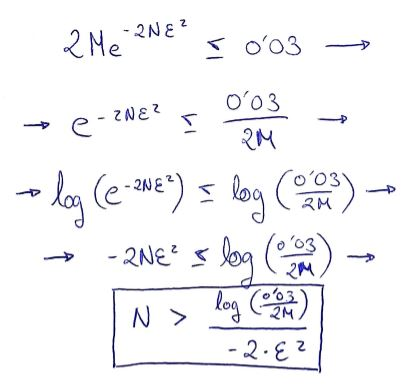
\includegraphics[scale=0.80]{imagenes/1} 
\end{figure}

Una vez despejada, simplemente aplicamos los valores que nos dan en el ejercicio para obtener las cantidades mínimas de N.
Primeramente con M = 1:

\begin{figure}[H] %con el [H] le obligamos a situar aquí la figura
	\centering
	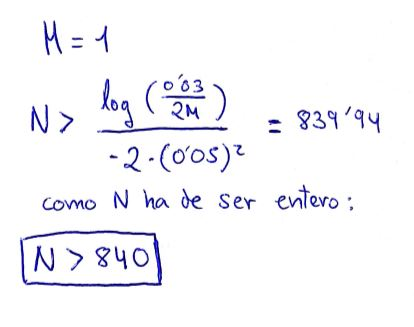
\includegraphics[scale=0.80]{imagenes/2} 
\end{figure}

Seguimos con M = 10.

\begin{figure}[H] %con el [H] le obligamos a situar aquí la figura
	\centering
	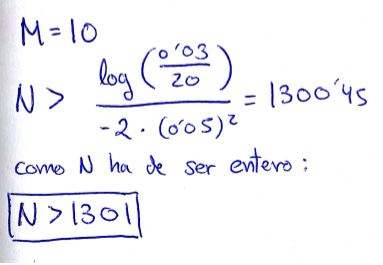
\includegraphics[scale=0.80]{imagenes/3} 
\end{figure}

Terminamos con M = 100

\begin{figure}[H] %con el [H] le obligamos a situar aquí la figura
	\centering
	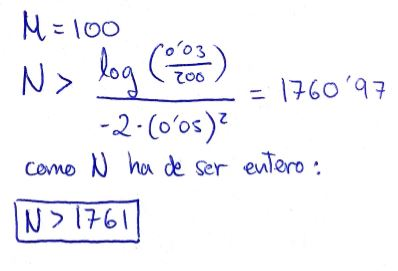
\includegraphics[scale=0.80]{imagenes/4} 
\end{figure}



\section{El jefe de investigación de una empresa con mucha experiencia en problemas de predicción de datos tras analizar los resultados de los muchos algoritmos de aprendizaje usados sobre todos los problemas en los que la empresa ha trabajado a lo largo de su muy dilatada existencia, decide que para facilitar el mantenimiento del código de la empresa van a seleccionar un único algoritmo y una única clase de funciones con la que aproximar todas las soluciones a sus problemas presentes y futuros. ¿Considera que dicha decisión es correcta y beneficiará a la empresa? Argumentar la respuesta usando los resultados teóricos estudiados.
}

Pienso que es una mala decisión debido a la existencia de una gran cantidad de problemas distintos, esta es la idea principal de mi argumento.\\

El propio uso de un único algoritmo no tiene por que dar problemas más allá de los tiempos de ejecución que, al no ser un algoritmo de un problema específico, puede que demore una cantidad mayor de tiempo al ser ejecutado pero poco más.\\
 En cambio el uso de una sola clase de funciones (H) con las que aproximar todas las soluciones a sus problemas es probable que de problemas, estos pueden presentarse de dos tipos:

\begin{enumerate}
	\item En caso de escoger un conjunto H de tamaño reducido, el rango de problemas resolubles será pequeño, es decir, si quiero resolver un problema X con un conjunto de funciones H pequeño y la solución de dicho problema se encuentra incluida en ese conjunto, entonces ese problema será resuelto de forma óptima pero, en caso de que la solución de tal problema no se halle en el conjunto H, este no será resuelto de manera óptima, o puede que ni tan siquiera sea resuelto.
	\item Por el lado contrario si hacemos el conjunto H grande, incrementamos la cantidad de problemas que pueden ser resueltos pero a su vez, disminuimos la probabilidad de que sea resuelto de forma óptima, ya que estamos generalizando una clase de funciones para la resolución de problemas de diversos tipos.
\end{enumerate}

En caso de tener que escoger una u otra opción a la fuerza, para empresas que se dedican a la resolución de problemas de una amplia gama de tipos, sería recomendable tener un conjunto H grande con el que poder resolver muchos problemas. Por otro lado, para empresas cuyo objetivo sea resolver problemas específicos con una precisión considerable, es recomendable usar un conjunto H pequeño.



\section{Para un conjunto H con dvc = 10  ¿que tamaño muestral se necesita (según la cota de generalización)  para tener un 95\% de confianza de que el error de generalización sea como mucho 0.05?}

\begin{figure}[H] %con el [H] le obligamos a situar aquí la figura
	\centering
	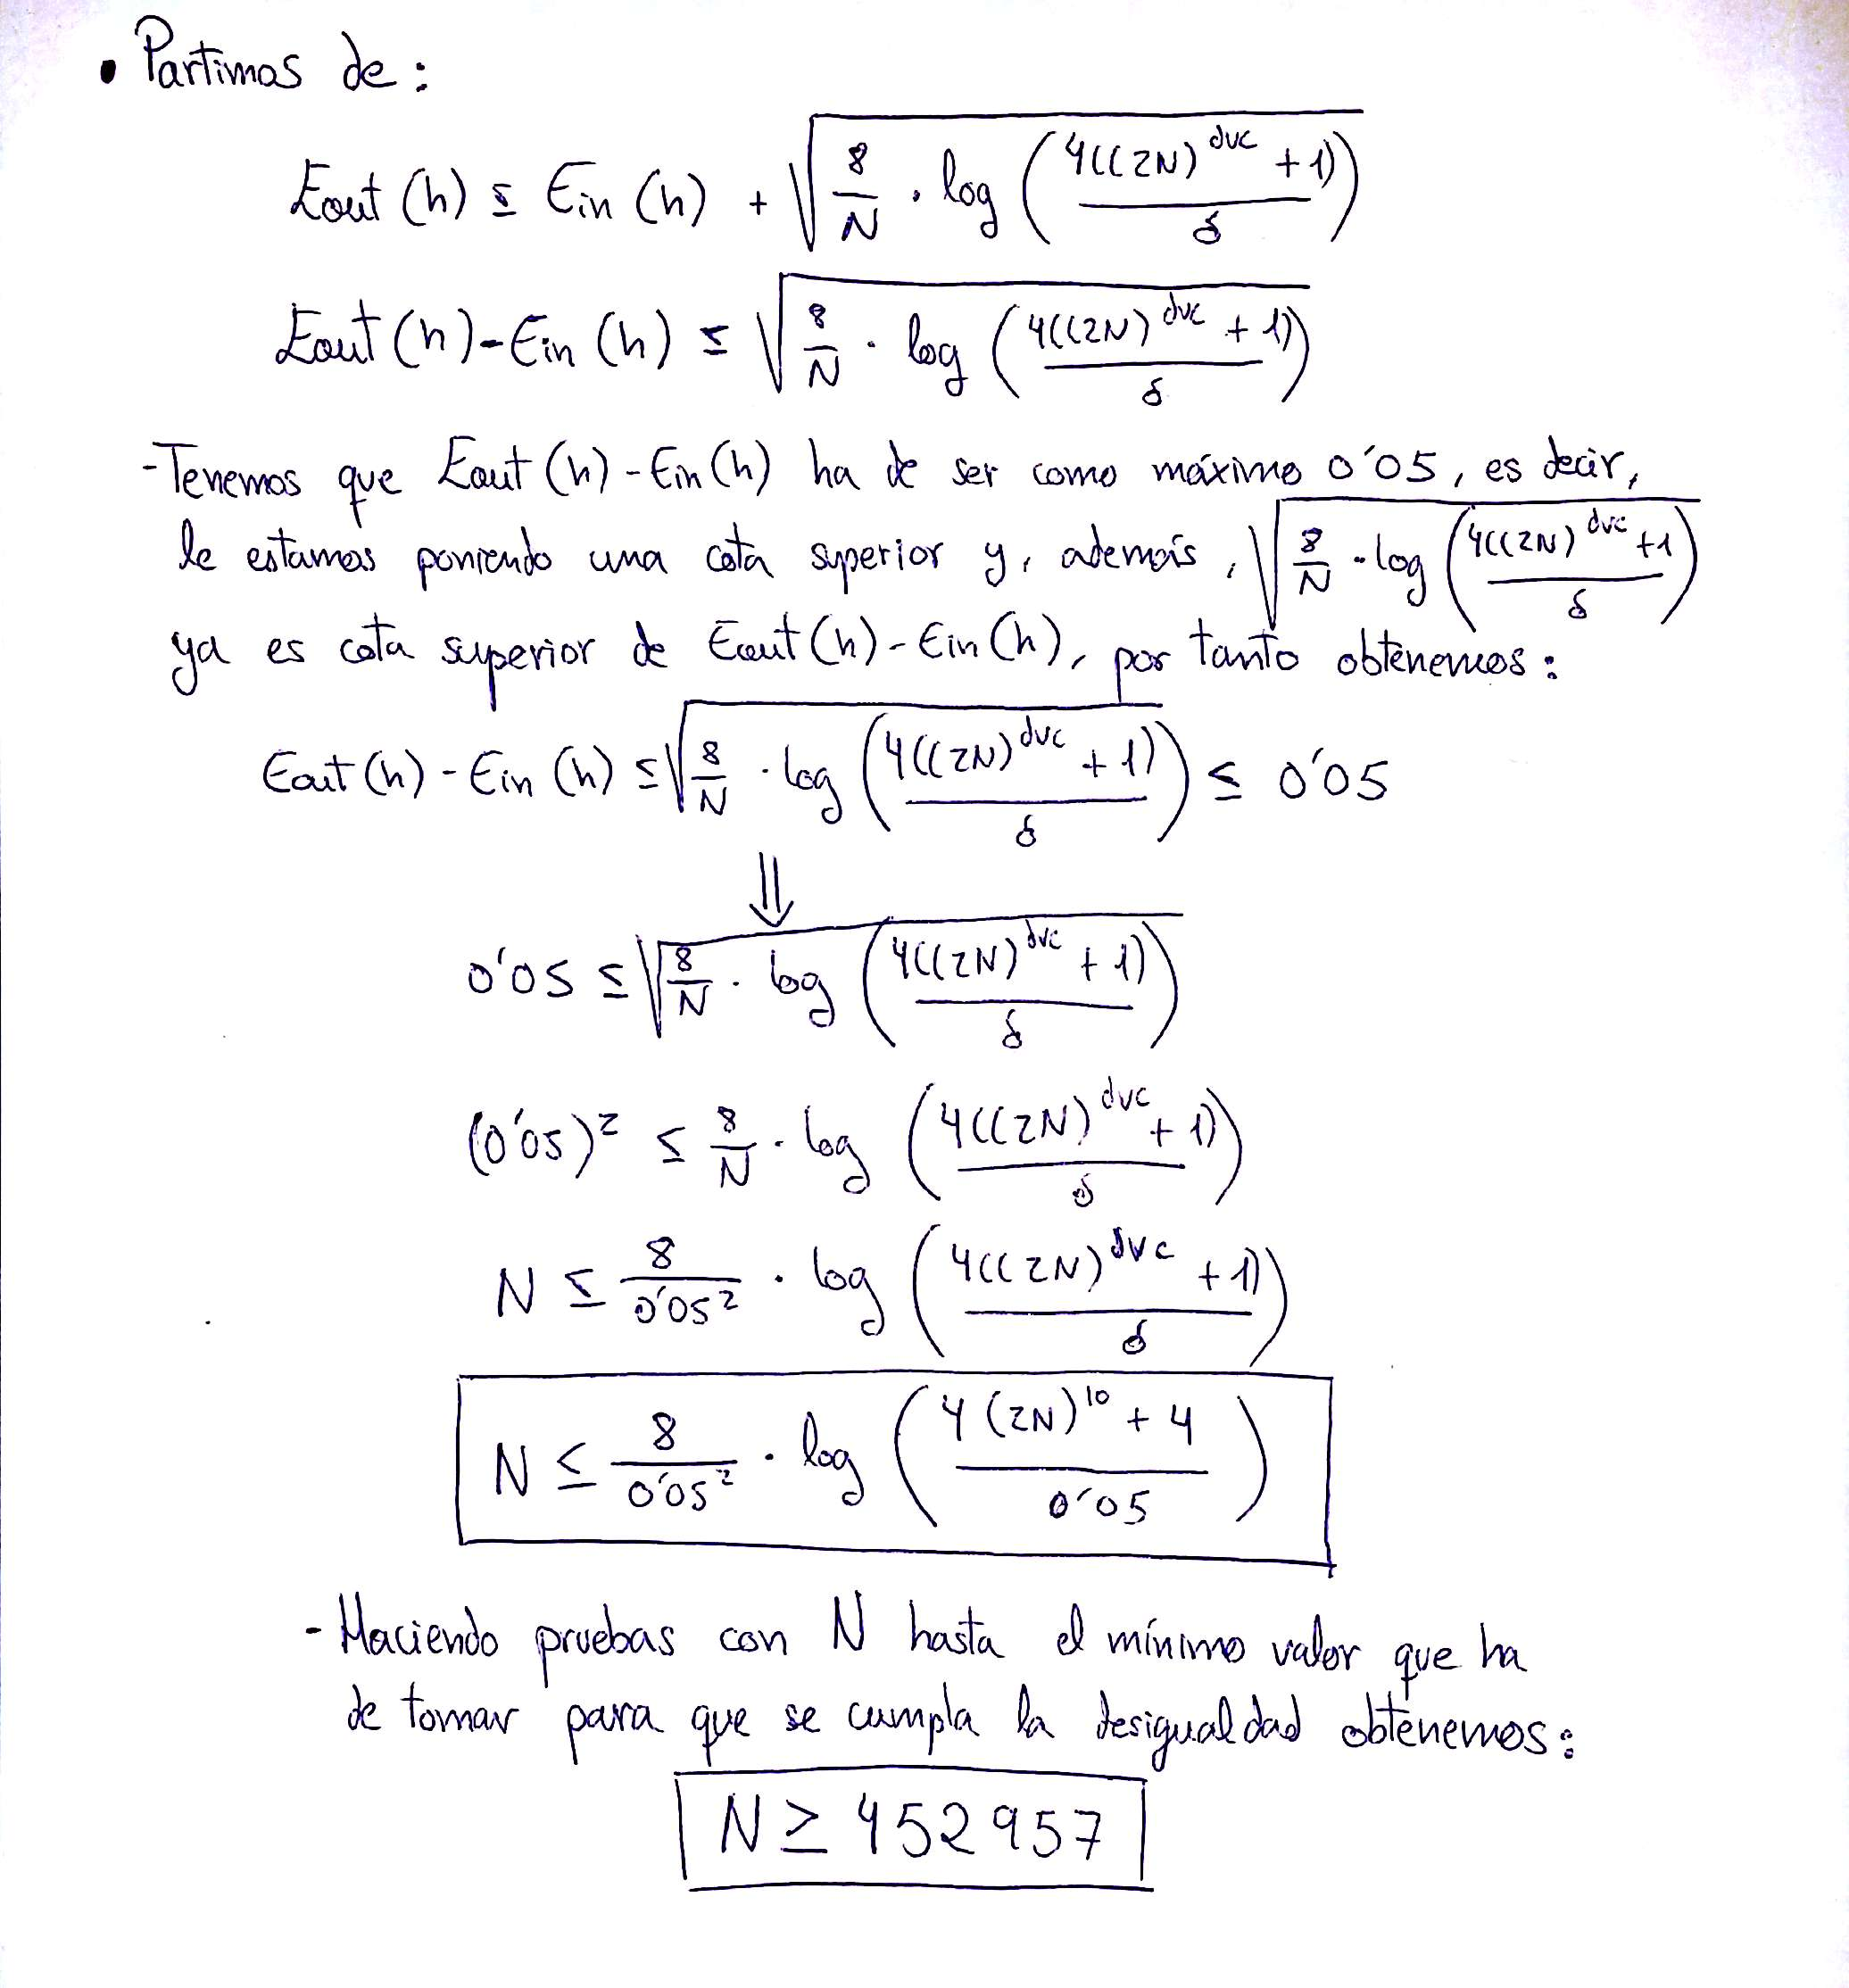
\includegraphics[scale=0.230]{imagenes/5} 
\end{figure}





\section{ Identificar de forma precisa las dos condiciones que garantizan que un problema de predicción puede ser aproximado por inducción desde una muestra de datos y una clase de funciones. Justificar la respuesta usando los resultados teóricos estudiados.}

Condiciones que garantizan que un problema de predicción puede ser aproximado por inducción desde una muestra de datos y una clase de funciones:

\begin{enumerate}
	\item Para que Eout(h) - Ein(h) tienda a cero, el tamaño de la muestra N ha de ser lo suficientemente grande para que en la ecuación de la cota de Vapnik\&Chervonenkis, log(N)/N tienda a 0 (debido al crecimiento más rápido de N). Si eso tiende a cero, entonces Eout(h)-Ein(h) será un valor muy parecido a 0, lo que indicará que el error dentro de la muestra será prácticamente igual que el error fuera de la muestra.
	\item dVc (la dimensión de Vapnik\&Chervonenkis) ha de ser finita. En caso de no serla(tiende a infinito) podemos observar en la misma ecuación que Eout-Ein no tiene cota superior, por lo que se nos puede presentar el caso de que el error dentro de la muestra sea muy inferior al error existente fuera de la muestra, cosa que para nada nos interesa.
\end{enumerate}

\newpage
\section{Considere que le dan una nuestra de tamaño N de datos etiquetados {-1,+1} y le piden que encuentre la función que mejor ajuste dichos datos. Dado que desconoce la verdadera función f, discuta los pros y contras de aplicar los principios de inducción ERM y SRM para lograr el objetivo. Valore las consecuencias de aplicar cada uno de ellos.
}



\textbf{ERM}

Como pro puede decirse que la cota no depende de la naturaleza de los datos de la muestra, tan sólo depende de la cantidad que hay(N). Como contra tenemos que ERM no siempre garantiza el aprendizaje si se cumple que N/dVC < 20. \\

\textbf{SRM}

A favor de la regla de inducción SRM podemos mencionar que busca directamente la minimización del Eout en lugar del Ein como hace ERM. En su contra que diferentes algoritmos pueden darnos diferentes funciones g aproximadas a f aún siendo aplicadas al mismo conjunto H. Este hecho depende del algoritmo usado y del conjunto de funciones H.
\newpage








\newpage
%------------------------------------------------

\bibliography{citas} %archivo citas.bib que contiene las entradas 
\bibliographystyle{plain} % hay varias formas de citar




\end{document}
